\documentclass[a4paper]{article}
\usepackage[14pt]{extsizes}
\usepackage[utf8]{inputenc}
\usepackage[T2A]{fontenc}
\usepackage{amssymb,amsmath,mathtext}
\usepackage{indentfirst,amsfonts}
\usepackage[english, russian]{babel}
\usepackage{setspace}
\usepackage{graphicx}
\usepackage{pscyr}
\usepackage{booktabs}
\usepackage[left=30mm, top=20mm, right=10mm, bottom=20mm, nohead, footskip=10mm]{geometry}
\usepackage{sectsty}
\usepackage{tocloft}
\renewcommand\cftsecfont{\mdseries}
\renewcommand\cftsecpagefont{\mdseries}
\graphicspath{{graphs/}}
\onehalfspacing
\renewcommand{\rmdefault}{ftm} % Times New Roman
\addto\captionsrussian{\renewcommand{\contentsname}{\normalfont Содержание}}
\addto\captionsrussian{\renewcommand{\refname}{\centering СПИСОК ИСПОЛЬЗОВАННЫХ ИСТОЧНИКОВ}}
\allsectionsfont{\normalfont}
\begin{document}
	%Титульный лист
	\begin{titlepage} % начало документа
	
	% НАЧАЛО ТИТУЛЬНОГО ЛИСТА
	\begin{center}
		\small{ФЕДЕРАЛЬНОЕ ГОСУДАРСТВЕННОЕ БЮДЖЕТНОЕ ОБРАЗОВАТЕЛЬНОЕ}\\ 
		УЧРЕЖДЕНИЕ ВЫСШЕГО ОБРАЗОВАНИЯ\\
		«МОСКОВСКИЙ ГОСУДАРСТВЕННЫЙ УНИВЕРСИТЕТ\\
		имени М.В.ЛОМОНОСОВА»\\
		\hfill \break
		ФИЗИЧЕСКИЙ ФАКУЛЬТЕТ \\
		\hfill \break
		КАФЕДРА МАТЕМАТИЧЕСКОГО МОДЕЛИРОВАНИЯ И ИНФОРМАТИКИ\\
		\hfill \break
		\hfill \break
		\hfill \break
		\hfill \break
		МАГИСТЕРСКАЯ ДИССЕРТАЦИЯ\\
		\hfill \break
		\textbf{<<РЕКОНСТРУКЦИЯ ТРЕХМЕРНЫХ ПОРИСТЫХ СРЕД С ИСПОЛЬЗОВАНИЕМ ИСКУССТВЕННЫХ НЕЙРОННЫХ СЕТЕЙ>>}\\
	\end{center}
	
	\hfill \break

	\begin{flushright}
		Выполнил студент \\
		235М группы:\\
		Будакян Я. С.\\
		\underline{\hspace{3cm}}\\
		\hfill \break
		Научный руководитель: \\
		к.т.н., доц. Грачев Е. А.\\
		\underline{\hspace{3cm}}
	\end{flushright}
	
	\begin{flushleft}
		Допущена к защите\\
		Зав. кафедрой \underline{\hspace{3cm}}\\
	\end{flushleft}
	\hfill \break
	\begin{center}
		Москва \\
		\hfill \break
		2019
	\end{center}
	
	\thispagestyle{empty} % выключаем отображение номера для этой страницы
	
	% КОНЕЦ ТИТУЛЬНОГО ЛИСТА

\end{titlepage}  % КОНЕЦ ДОКУМЕНТА !
	%Учет титульного листа в нумерации
	\setcounter{page}{2}
	\tableofcontents
	\addcontentsline{toc}{section}{ВВЕДЕНИЕ}
	% ВВЕДЕНИЕ
	\clearpage
\section*{\hfil ВВЕДЕНИЕ \hfil}
	ВВЕДЕНИЕ
	% Нейронные сети
	\clearpage
\section{Нейронные сети}
	ИНС - искусственная нейронная сеть - это математическая модель, построенная по принципу организации и функционирования биологических нейронных сетей. Она представляет собой систему соединённых простых блоков - искусственных нейронов, каждый из которых имеет входы и выходы для взаимодействия с другими нейронами. Главное преимущество нейронных сетей перед традиционными алгоритмами в том, что они обучаются на некотором наборе данных, а не программируются в классическом смысле этого понятия. Процесс обучения заключается в нахождении оптимальных весовых коэффициентов между нейронами. С математической точки зрения, процесс обучения - это задача многопараметрической нелинейной оптимизации.
	\subsection{Математическая модель нейрона}
		Одиночный нейрон обычно представляет собой взвешенный сумматор с нелинейной функцией активации на выходе:
		$$x_{out} = \phi(\vec{w} \cdotp \vec{x}_{in}),$$
		где $\vec{w}$ - вектор весовых коэффициентов связей, $\vec{x}_{in}$ - входной вектор, $\phi$ - нелинейная функция активации (Рис. \ref{3-artificial-neuron-model}).
		
		\begin{figure}[h]
			\centering{\includegraphics[width=0.95\linewidth]{3-ann/artificial-neuron-model}}
			\caption{Математическая модель нейрона}
			\label{3-artificial-neuron-model}
		\end{figure}
		
		Функции активации могут выбираться разными в зависимости от задачи. Наиболее часто используемые функции:
		
		\begin{itemize}
			\item Сигмоида (логистическая функция)
					$$\sigma(x) = \frac{1}{1 + e^{-x}}$$
			\item Гиперболический тангенс
			\item ReLU
					$$ReLU(x) = \max(0, x)$$
			\item softmax
					$$\sigma(\vec{x})_j = \frac{e^{x_j}}{\sum_{k=1}^{N} e^{z_k}}$$
		\end{itemize}
		Множество подобных нейронов соединяется в сеть и обучается с помощью метода обратного распространения ошибки вкупе с каким-либо методом численной оптимизации.
	\subsection{Метод обратного распространения ошибки}
		Метод обратного распространения ошибки (backpropagation) - самый широко используемый и успешный алгоритм обучения глубоких (многослойных) нейронных сетей. Суть метода заключается в распространении сигналов ошибки от выходов сети к ее входам в обратном к распространению сигнала в сети направлении. Это позволяет вычислить производные функционала ошибки по весам сети, которые потом можно использовать в любом градиентном алгоритме оптимизации (например, градиентном спуске).
		
		Обозначим множество входов сети как $\{x_1, \ldots, x_n\}$, множество выходов - $O$, $w_{ij}$ - вес, присвоенный ребру, соединяющему $i$-й и $j$-й узлы, $y_k$ - известные (правильные) ответы, $o_i$ - выход $i$-го узла. Введём функцию ошибки (например, сумма квадратов расстояний):
		$$ L(\vec{x}, W) = \frac{1}{2} \sum_{k \in O} (y_k - o_k)^2, $$
		где $W = \{w_{ij}\}$ - матрица весовых коэффициентов
		
		Рассмотрим сначала нейроны последнего слоя. Весовой коэффициент $w_{ij}$ влияет на выход сети как часть суммы $S_j = \sum_i w_{ij} x_i$. Соответственно,
		$$ \frac{\partial L}{\partial w_{ij}} = \frac{\partial L}{\partial S_j} \frac{\partial S_j}{\partial w_{ij}} = x_i \frac{\partial L}{\partial S_j} $$
		
		Аналогично, $S_j$ влияет на общую ошибку только в рамках выхода $j$-го узла $o_j$, поэтому
		$$ \frac{\partial L}{\partial S_j} = \frac{\partial L}{\partial o_j} \frac{\partial o_j}{\partial S_j}  = \left(\frac{\partial}{\partial o_j} \frac{1}{2} \sum_{k \in Out} (y_k - o_k)^2 \right) \left(\frac{\partial \phi(S)}{\partial S} \bigg|_{S = S_j} \right)$$
		Если узел $j$ не находится на последнем слое, то у него есть набор связей с нейронами следующего слоя. Обозначим их множество как $K_j$. Тогда
		$$ \frac{\partial L}{\partial S_j} = \sum_{k \in K_j} \frac{\partial L}{\partial S_k} \frac{\partial S_k}{\partial S_j} $$
		$$ \frac{\partial S_k}{\partial S_j} = \frac{\partial S_k}{\partial o_j} \frac{\partial o_j}{\partial S_j} = w_{jk}\frac{\partial o_j}{\partial S_j} $$
		$ \frac{\partial L}{\partial S_k}$ - аналогичная поправка, но для нейрона следующего слоя. В итоге, получены выражения для производных ошибки по весам для нейронов выходного слоя, а аналогичные производные для нейронов внутренних слоев выражены через нейроны следующих слоев. Это и есть процесс обратного распространения ошибки - градиенты ошибки по весам вычисляются последовательно, начиная с выходного слоя и заканчивая первым.
	\subsection{Сверточные нейронные сети}
		Сверточные нейронные сети (CNN - convolutional neural networks) - это специальная архитектура нейронной сети, нацеленная на эффективное распознавание изображений, впервые предложенная Яном Лекуном \cite{LeCun}. Структура такой сети имеет некоторое сходство со строением зрительной коры головного мозга. Свое название CNN получили из-за наличия сверточных слоев, в которых каждый фрагмент изображения умножается на ядро свертки, полученный результат суммируется и записывается в аналогичную позицию выходного изображения. Одно отдельное ядро свертки обычно интерпретируют как кодирование какого-либо признака изображения. При этом сами ядра выучиваются сетью самостоятельно, а не закладываются человеком. В CNN чередуются сверточные и субдискретизирующие слои, таким образом более глубокие сверточные слои могут выделять абстрактные детали изображения, вплоть до общих понятий, таких как ``кошка'', ``собака'', и т.п. На данный момент CNN являются наиболее популярным алгоритмом машинного обучения при работе с изображениями.
	\subsection{Генеративные состязательные сети}
		Архитектура нейронной сети, получившая название генеративной состязательной сети (generative adversarial network - GAN), впервые была описана в 2014 году \cite{Goodfellow}. За последнее время сети такого типа добились больших успехов в задачах синтеза объектов из сложных распределений. Этим объясняется мотивация попытки применения данной архитектуры для решения поставленной задачи.
		\subsubsection{Общая структура}
			Переформулируем изначальную задачу нахождения процедуры синтеза $X'$ такой что $ P_{X'} \approx P_X$:
			$$ \rho(P_{X'}, P_X) \longrightarrow \underset{P_{X'}}{\min} $$
			Введём параметризированную процедуру генерации:
			$$ X' = g_{\theta}(\cdot) $$
			Получаем:
			$$ \rho(P_{X'}, P_X) \longrightarrow \underset{P_{X'}}{\min} $$
			$$ \rho(g_{\theta}(\cdot), P_X) \longrightarrow \underset{g_{\theta}(\cdot)}{\min} $$
			$$ \rho(g_{\theta}(\cdot), P_X) \longrightarrow \underset{\theta}{\min} $$
			В данном случае $\rho$ выступает некоторой метрикой похожести двух вероятностных распределений.
			Идея GAN заключается в том, что в качестве такой метрики используется функционал ошибки другой нейросети -  обученного классификатора: чем чаще ошибается обученный классификатор, тем больше одно распределение похоже на другое. Тогда задача принимает вид:
			$$ \rho(P_{X'}, P_X) \longrightarrow \min \Leftrightarrow L \longrightarrow \max, $$
			где $L$ - функция потерь обученного классификатора.
			Соответственно, вводятся две нейросети:
	
			\begin{itemize}
				\item $d_{\zeta}(x)$ - классификатор для оценки $\rho$, ``дискриминатор''
				\item $g_{\theta}(x)$ - сеть, трансформирующая шум в элементы множества $X'$, ``генератор''
			\end{itemize}
	
			Суть использования двух сетей состоит в том, что они обучаются совместно, конкурируя друг с другом: генератор пытается имитировать целевое распределение, а дискриминатор классифицирует поступающие от генератора и из обучающей выборки изображения на 2 класса: реальные (из изначального распределения $P_X$) и ложные (из $P_{X'}$, т.е. синтезированные генератором). Сигнал от дискриминатора возвращается в генератор и используется для обучения генератора ``обману'' дискриминатора.
			Для дальнейшего рассмотрения введём функцию потерь дискриминатора (BCE - binary cross-entropy, logloss):
			$$ l_1 = l(d_{\zeta}(x), 1) $$
			$$ l_2 = l(d_{\zeta}(x'), 0) $$
			$$ L(X, X') = \frac{1}{2} \mathbb{E}_{X} l_1 + \frac{1}{2} \mathbb{E}_{X'} l_2 = -\frac{1}{2} (\mathbb{E}_{X} \log d_{\zeta}(x) + \mathbb{E}_{X'} \log (1 - d_{\zeta}(x'))) = $$
			$$ =  -\frac{1}{2} (\mathbb{E}_{X} \log d_{\zeta}(x) + \mathbb{E}_{V} \log (1 - d_{\zeta}(g_{\theta}(v)))) = L(\zeta, \theta) .$$
			Функция потерь обученного классификатора:
			$$ L^*(\theta) = \underset{\zeta}{\min} L(\zeta, \theta) $$
			Соответственно,
			$$ \underset{\zeta}{\min} L(\zeta, \theta) \longrightarrow \underset{\theta}{\max} $$
			$$ \theta^* = \underset{\theta}{\arg\max} \left[ \underset{\zeta}{\min} L(\zeta, \theta) \right] $$
			Определим оптимальный дискриминатор:
			$$ d^*_{\theta} = d_{\zeta^*(\theta)} $$
			$$ \zeta^*(\theta) =  \underset{\zeta}{\arg\min} L(\zeta, \theta)$$
			
		\subsubsection{Обучение GAN}
			Итак, задача обучения GAN свелась к нахождению оптимальных весов генератора
			$$ \theta^* = \underset{\theta}{\arg\max} \left[ \underset{\zeta}{\min} L(\zeta, \theta) \right] $$
			Процесс обучения такой системы сетей принимает итеративный вид:
	
			\begin{itemize}
				\item Обучается дискриминатор при фиксированном генераторе
				\item Обучается генератор при фиксированном дискриминаторе
				\item Повторяется до сходимости параметров обеих моделей
			\end{itemize}
			Описанный процесс схематично изображён на (Рис. \ref{2-gan-training}).
	
			\begin{figure}[h!]
				\centering{\includegraphics[width=0.4\linewidth]{3-ann/gan-training}}
				\caption{Схематическое изображение процесса обучения GAN}
				\label{2-gan-training}
			\end{figure}
	
		\subsubsection{Модификации ``DCGAN'' и ``3D-DCGAN''}
			Модификация архитектуры GAN под названием DCGAN \cite{Radford} была предложена в 2015 году и совершила прорыв в области синтеза изображений. Суть архитектуры заключается в нескольких принципах построения сетей и их обучания. Во-первых, использование свёрточных слоев и пакетной нормализации (batch normalization)  как в генераторе, так и дискриминаторе. В генераторе, при этом, используются специальные обратные свёрточные слои (transposed convolution, deconvolution). Во-вторых, использование специальной функции активации в дискриминаторе - $LeakyReLU$:
			\[ LeakyReLU(x) = \left \{ \begin{array}{rcl} 0.01 x & \mbox{for} & x < 0\\ x & \mbox{for} & x \ge 0\end{array} \right .\]  
			Все эти идеи позволяют стабилизировать сложный процесс обучения GAN и увеличить качество синтезируемых объектов.
			
			Архитектура 3D-DCGAN совмещает в себе идеи \cite{Radford} и \cite{Wu}. Основное отличие от обычной DCGAN состоит в том, что вместо двухмерных свёрток во всех свёрточных слоях сетей используются трёхмерные, что и позволяет реконструировать трёхмерные среды.
			
			Авторы \cite{Mosser} используют 3D-DCGAN для реконструкции пористых сред. Схема процесса обучения показана на (Рис. \ref{2-gan-scheme})
			
			\begin{figure}[h!]
				\centering{\includegraphics[width=0.8\linewidth]{3-ann/GAN_overview}}
				\caption{Схема процесса обучения}
				\label{2-gan-scheme}
			\end{figure}
		
			Обучение 3D-GAN сводится к минимизации функционала:
			\[ \underset{\theta}{\min} \underset{\zeta}{\max} \ \mathbb{E}_{x \sim p_{data}}\log D_\zeta(x) + \mathbb{E}_{z \sim p_{z}} \log (1 - D_\zeta(G_\theta(z))) \]
		
		\subsubsection{Модификация процедуры обучения}
			Сеть, использованная в этой работе, полностью повторяет архитектуру сетей \cite{Mosser}, однако в процедуру обучения сетей внесена модификация.
			
			Скорость обучения - один из наиболее важных гиперпараметров (параметров, которые задаются человеком, а не оптимизируются в ходе процесса обучения). Её значение может радикально влиять на весь процесс сходимости сети \cite{Smith}. В \cite{Mosser} авторы вручную управляют значением скорости обучения, изменяя её в зависимости от рассчитанных функционалов Минковского и визуальной структуры реконструируемых образцов. Это видно на графике профиля обучения сетей, приведённом в \cite{Mosser} (Рис. \ref{2-berea-curve}):
			
			\begin{figure}[h!]
				\centering{\includegraphics[width=1\linewidth]{3-ann/berea_training_curve}}
				\caption{Схема процесса обучения \cite{Mosser}}
				\label{2-berea-curve}
			\end{figure}
		
			В этой работе исследуется применение модификации процедуры обучения, которая состоит в том, что:
			
			\begin{itemize}
				\item Значения функционалов Минковского рассчитываются для реконструированных образцов на каждой итерации процесса обучения, что позволяет отслеживать текущее состояние сети-генератора с точки зрения совпадения топологических характеристик образцов с желаемыми;
				\item Это позволяет после каждого шага обучения оценить невязку $\Delta_i$:
					\[ \Delta_i = |B_i - B_{berea}| + |\xi_i - \xi_{berea}|, \]
					где $B_i$, $\xi_i$ - это значения соответствующих функционалов Минковского для реконструированного образца с помощью генератора на текущем шаге обучения, а $B_{berea}$ и $\xi_{berea}$ - значения этих функционалов для исходного образца.
			\end{itemize}
			Если значение $\Delta_i$ не меняется более 3000 итераций, то скорость обучения уменьшается в 10 раз.
	% Численная оптимизация
	\clearpage
\section{Градиентные методы оптимизации}
	Для обучения глубоких нейросетей применяется метод обратного распространения ошибки, который позволяет рассчитать градиенты весов, и различные алгоритмы численной оптимизации. В данной работе для обучения моделей применялся алгоритм оптимизации ``Adam'', являющийся модификацией стохастического градиентного спуска (SGD).
	\subsection{Градиентный спуск}
		Обычный градиентный спуск - простой итеративный алгоритм численной оптимизации. Для минимизации целевой функции рассчитывается ее градиент в этой точке, после чего совершается шаг в сторону антиградиента, т.е. из текущего значения параметра вычитается градиент целевой функции по данному параметру, умноженный на гиперпараметр $\lambda$ - скорость обучения.
		$$ \theta_{t+1} = \theta_t - \lambda \nabla L(\theta_t), $$
		где $L$ - целевая функция.
	\subsection{Стохастический градиентный спуск}
		Описание стохастического градиентного спуска есть в \cite{Amari}. Стохастический градиентый спуск отличается от обычного тем, что градиент целевой функции подсчитывается не на всем наборе данных, а на его случайном подмножестве. Это широко используется при обучении нейронных сетей, поскольку высчитывание полного градиента функции ошибки по всем параметрам (используя всю обучающую выборку) приводит к слишком высоким временным затратам.
		$$ i \sim \mathcal{U}\{1, 2, ..., n\} $$
		$$ \theta_{t+1} = \theta_t - \lambda \nabla L_i(\theta_t), $$
		где $L_i$ - целевая функция, вычисленная на $i$-ой части данных (mini-batch, мини-пакет), индекс $i$ выбирается случайно.
		\subsubsection{RMSprop}
			RMSprop (root mean square propagation) описан в \cite{Hinton}. Идея заключается в том, что для каждого параметра градиент перемасштабируется, учитывая прошлые значения градиентов для этого параметра. Производится это с помощью деления градиента на нормировочный множитель - корень из среднего квадрата градиентов.
			$$ g_{t+1} = \gamma g_t + (1 - \gamma) (\nabla L_i(\theta_t))^2$$
			$$ \theta_{t+1} = \theta_t - \frac{\lambda \nabla L_i(\theta_t)}{\sqrt{g_{t+1} + \epsilon}}, $$
			где $\epsilon$ - это небольшая константа, введённая для численной стабильности.
		\subsubsection{Adam}
			Adam (adaptive moment estimation, описан в \cite{Kingma}). Этот алгоритм, помимо перемасшабирования, использует инерцию градиента, что позволяет смягчить быстрое изменение градиента, присущее стохастическому градиентному спуску.
			$$ m_{t+1} = \beta_1 m_t + (1 - \beta_1) \nabla L_i(\theta_t) $$
			$$ v_{t+1} = \beta_2 g_t + (1 - \beta_2) (\nabla L_i(\theta_t))^2 $$
			$$ \hat{m_t} = \frac{m_t}{1 - \beta_1^t} $$
			$$ \hat{v_t} = \frac{v_t}{1 - \beta_2^t}$$
			$$ \theta_{t+1} = \theta_t - \frac{\lambda \hat{m_t}}{\sqrt{v_t + \epsilon}} $$
			Авторы статьи \cite{Kingma} пишут, что этот алгоритм достаточно устойчив к неоптимальному выбору параметров, поэтому во многих статьях в начале для обучения пробуют применить именно Adam.
	% Верификация
	\clearpage
\section{Верификация}

	Верификация синтеза
	
	\subsection{Функционалы Минковского}
		Функционалы Минковского для трехмерных тел вводятся следующим образом:
		\begin{itemize}
			\item $ \displaystyle V = M_0 = \int_{X} dV $
			\item $ \displaystyle S = M_1 = \frac{1}{3} \int_{\delta X} dS $
			\item $ \displaystyle B = M_2 = \frac{1}{6} \int_{\delta X} \left ( \frac{1}{R_1} + \frac{1}{R_2} \right ) dS$
			\item $\displaystyle \xi = M_3 = \frac{1}{3} \int_{\delta X} \frac{1}{R_1 R_2} dS $
		\end{itemize}
	
		+ теория
	
		\subsubsection{Расчет для дискретного случая}
			Алгоритм расчета функционалов Минковского в дискретном случае: []
	
	\subsection{Двухточечная корреляционная функция}
		
		+ теория
		
	% ВЫВОДЫ
	\clearpage
\section{Результаты вычислительного эксперимента}
	Архитектуры нейронных сетей, а также модификация процедуры обучения, описанные в пунктах 1.4.3 и 1.4.4 были реализованы в виде комплекса программ на языке Python с помощью библиотеки для глубокого обучения PyTorch. Использованные версии программных пакетов указаны в Приложении 1. Обучение проводилось на наборе данных Berea.
	
	\subsection{Набор данных Berea}
		Исходные данные - изображение компьютерной томографии песчаника, объёмом $400^3$ вокселей, бинарно сегментированная на породу и поры, в формате TIFF. Разрешение томограммы равно 3 микрометрам. Для обучения сетей из этого кубика был вырезан набор кубиков размером $64^3$ вокселей, с перекрытием в 16 вокселей (всего 10648 различных образцов размера $64^3$), они и представили собой обучающую выборку. Оригинальный образец размером $400^3$ вокселей представлен на (Рис. \ref{5-full-berea}). Некоторые примеры из получившейся обучающей выборки представлены в (Таб. \ref{5-berea64}).
		
		\begin{figure}[h]
			\centering{\includegraphics[width=0.6\linewidth]{5-results/berea/original}}
			\caption{Оригинальный образец}
			\label{5-full-berea}
		\end{figure}
	
		\begin{table}[h]
			\centering
			\begin{tabular}{p{5cm} p{5cm} p{5cm}}
				\toprule
				\includegraphics[width=1.0\linewidth]{5-results/berea/berea_1}
				&
				\includegraphics[width=1.0\linewidth]{5-results/berea/berea_2}
				&
				\includegraphics[width=1.0\linewidth]{5-results/berea/berea_3}
				\\
				\includegraphics[width=1.0\linewidth]{5-results/berea/berea_4}
				&
				\includegraphics[width=1.0\linewidth]{5-results/berea/berea_5}
				&
				\includegraphics[width=1.0\linewidth]{5-results/berea/berea_6}
				\\
				\bottomrule
			\end{tabular}
			\caption{Примеры из обучающей выборки}
			\label{5-berea64}
		\end{table}
	\subsection{Обучение нейросети}
		Было проведено обучение нейросети со следующими параметрами (число свёрточных фильтров указано для первого слоя):
		\begin{table}[h]
			\centering
			\begin{tabular}{|c|c|c|c|}
				\hline
				Число фильтров G, D & Размерность z & Размер пакета & Начальный LR \\
				\hline
				64, 32 & 512 & 64 & 2e-4 \\
				\hline
			\end{tabular}
			\caption{Гиперпараметры нейросети и процесса обучения}
		\end{table}
	
		Итоговые архитектуры использованных нейронных сетей генератора и дискриминатора указаны в (Таб. \ref{5-g-arch}, \ref{5-d-arch})
		\begin{table}[h]
			\tabcolsep=0.11cm
			\centering
			\begin{tabular}{|c|c|c|c|}
				\hline
				Слой & Размер ядра & Размерность выхода & Кол-во параметров \\
				\hline
				0\_ConvTranspose3d &  [256, 512, 4, 4, 4] & [1, 256, 4, 4, 4] & 8 388 610 \\
				1\_BatchNorm3d &  [256] & [1, 256, 4, 4, 4] & 512 \\
				2\_ReLU & - & [1, 256, 4, 4, 4] & - \\
				\hline
				3\_ConvTranspose3d &  [128, 256, 4, 4, 4] & [1, 128, 8, 8, 8] & 2 097 150 \\
				4\_BatchNorm3d &  [128] & [1, 128, 8, 8, 8] & 256 \\
				5\_ReLU & - & [1, 128, 8, 8, 8] & - \\
				\hline
				6\_ConvTranspose3d &  [64, 128, 4, 4, 4] & [1, 64, 16, 16, 16] & 524 290 \\
				7\_BatchNorm3d &  [64] & [1, 64, 16, 16, 16] & 128 \\
				8\_ReLU & - & [1, 64, 16, 16, 16] & - \\
				\hline
				9\_ConvTranspose3d &  [32, 64, 4, 4, 4] & [1, 32, 32, 32, 32] & 131 070 \\
				10\_BatchNorm3d &  [32] & [1, 32, 32, 32, 32] & 64 \\
				11\_ReLU & - & [1, 32, 32, 32, 32] & - \\
				\hline
				12\_ConvTranspose3d &  [1, 32, 4, 4, 4] & [1, 1, 64, 64, 64] & 2 050 \\
				13\_Tanh & - & [1, 1, 64, 64, 64] & - \\
				\hline
			\end{tabular}
			\caption{Архитектура генератора}
			\label{5-g-arch}
		\end{table}
	
		\begin{table}[h]
			\tabcolsep=0.11cm
			\centering
			\begin{tabular}{|c|c|c|c|}
				\hline
				Слой & Размер ядра & Размерность выхода & Кол-во параметров \\
				\hline
				0\_Conv3d &  [1, 32, 4, 4, 4] & [1, 32, 32, 32, 32] & 2 050 \\
				1\_LeakyReLU & - & [1, 32, 32, 32, 32] & - \\
				\hline
				2\_Conv3d &  [32, 64, 4, 4, 4] & [1, 64, 16, 16, 16] & 131 070 \\
				3\_BatchNorm3d &  [64] & [1, 64, 16, 16, 16] & 128 \\
				4\_LeakyReLU & - & [1, 64, 16, 16, 16] & - \\
				\hline
				5\_Conv3d &  [64, 128, 4, 4, 4] & [1, 128, 8, 8, 8] & 524 290 \\
				6\_BatchNorm3d &  [128] & [1, 128, 8, 8, 8] & 256 \\
				7\_LeakyReLU & - & [1, 64, 16, 16, 16] & - \\
				\hline
				8\_Conv3d &  [128, 256, 4, 4, 4] & [1, 256, 4, 4, 4] & 2 097 150 \\
				9\_BatchNorm3d &  [256] & [1, 256, 4, 4, 4] & 512 \\
				10\_LeakyReLU & - & [1, 256, 4, 4, 4] & - \\
				\hline
				11\_Conv3d &  [256, 1, 4, 4, 4] & [1, 1, 1, 1, 1] & 16 380 \\
				12\_Sigmoid & - & [1, 1, 1, 1, 1] & - \\
				\hline
			\end{tabular}
			\caption{Архитектура дискриминатора}
			\label{5-d-arch}
		\end{table}
		
		Графики функций ошибок сетей генератора и дискриминатора, а также графики сходимостей функционалов Минковского в процессе обучения приведены на (Рис. \ref{loss-plot}, \ref{V-plot}, \ref{S-plot}, \ref{B-plot}, \ref{Xi-plot}).
		
		\begin{figure}[h]
			\centering{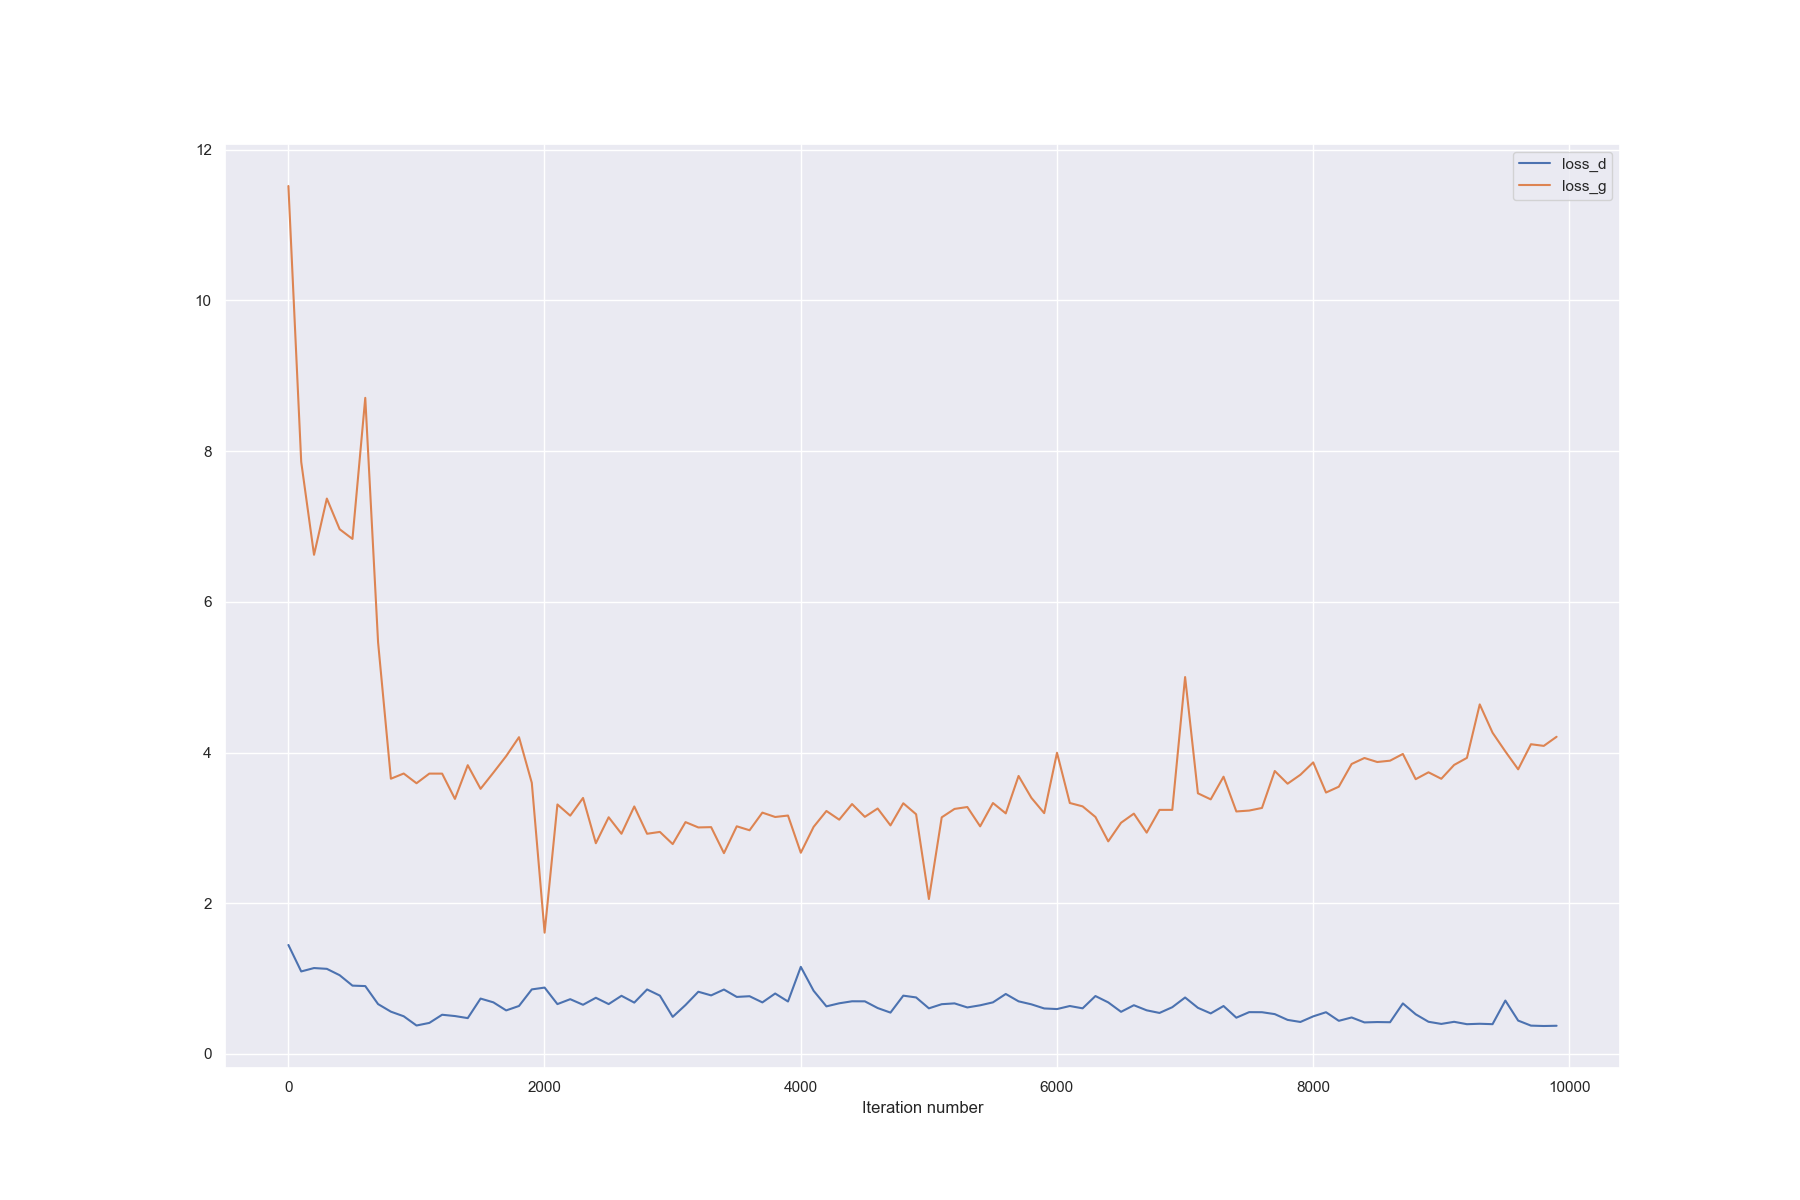
\includegraphics[width=0.95\linewidth]{5-results/experiment/loss_plot}}
			\caption{График функций ошибок сетей дискриминатора и генератора}
			\label{loss-plot}
		\end{figure}
	
		\begin{figure}[h]
			\centering{\includegraphics[width=0.95\linewidth]{5-results/experiment/minkowski_V_plot}}
			\caption{График сходимости функционала Минковского $V$}
			\label{V-plot}
		\end{figure}
		
		\begin{figure}[h]
			\centering{\includegraphics[width=0.95\linewidth]{5-results/experiment/minkowski_S_plot}}
			\caption{График сходимости функционала Минковского $S$}
			\label{S-plot}
		\end{figure}
	
		\begin{figure}[h]
			\centering{\includegraphics[width=0.95\linewidth]{5-results/experiment/minkowski_B_plot}}
			\caption{График сходимости функционала Минковского $B$}
			\label{B-plot}
		\end{figure}
	
		\begin{figure}[h]
			\centering{\includegraphics[width=0.95\linewidth]{5-results/experiment/minkowski_Xi_plot}}
			\caption{График сходимости функционала Минковского $\xi$}
			\label{Xi-plot}
		\end{figure}	
		
	
	\subsection{Реконструкции размера $64^3$}
		\subsubsection{Примеры}
			Примеры реконструкций размера $64^3$, приведены в (Таб. \ref{5-gen-64}). Дополнительные примеры реконструкций приведены в Приложении 2 (Таб. \ref{8-gen-64}).
			
			\begin{table}[h]
				\centering
				\begin{tabular}{p{5cm} p{5cm} p{5cm}}
					\toprule
					\includegraphics[width=1\linewidth]{5-results/analysis_64/generated/1}
					&
					\includegraphics[width=1\linewidth]{5-results/analysis_64/generated/2}
					&
					\includegraphics[width=1\linewidth]{5-results/analysis_64/generated/3}
					\\
					\includegraphics[width=1\linewidth]{5-results/analysis_64/generated/4}
					&
					\includegraphics[width=1\linewidth]{5-results/analysis_64/generated/5}
					&
					\includegraphics[width=1\linewidth]{5-results/analysis_64/generated/6}
					\\
					\includegraphics[width=1\linewidth]{5-results/analysis_64/generated/7}
					&
					\includegraphics[width=1\linewidth]{5-results/analysis_64/generated/8}
					&
					\includegraphics[width=1\linewidth]{5-results/analysis_64/generated/9}
					\\
					\bottomrule
				\end{tabular}
				\caption{Примеры реконструкций 64x64x64}
				\label{5-gen-64}
			\end{table} 
		
		\subsubsection{Анализ реконструкций}
			Было реконструировано 1000 образцов размера $64^3$. На основе этого набора были получены распределения интересующих функционалов Минковского. Также, используя предоставленную обученную сеть \cite{Mosser}, было реконструировано 1000 образцов того же размера для сравнения распределений функционалов. Графики полученных распределений (вместе с соответствующим распределением на обучающей выборке) приведены на (Рис. \ref{5-dist-V-64}, \ref{5-dist-S-64}, \ref{5-dist-B-64}, \ref{5-dist-Xi-64}). Была рассчитана двухточечная функция вероятности для реконструированных образцов, образцов, полученных с помощью предобученной сети \cite{Mosser} и образцов из обучающей выборки. Её график приведён на (Рис. \ref{5-prob-64}).
			
			\begin{figure}[h]
				\begin{minipage}[h]{0.49\linewidth}
					\centering{\includegraphics[width=1\linewidth]{5-results/analysis_64/V_exp} \\ Обученная сеть}
				\end{minipage}
				\hfill
				\begin{minipage}[h]{0.49\linewidth}
					\centering{\includegraphics[width=1\linewidth]{5-results/analysis_64/V_paper} \\ Mosser et al. \cite{Mosser}}
				\end{minipage}
				\caption{Распределения функционала Минковского $V$ для реконструкций размера $64^3$}
				\label{5-dist-V-64}
			\end{figure}
		
			\begin{figure}[h]
				\begin{minipage}[h]{0.49\linewidth}
					\centering{\includegraphics[width=1\linewidth]{5-results/analysis_64/S_exp} \\ Обученная сеть}
				\end{minipage}
				\hfill
				\begin{minipage}[h]{0.49\linewidth}
					\centering{\includegraphics[width=1\linewidth]{5-results/analysis_64/S_paper} \\ Mosser et al. \cite{Mosser}}
				\end{minipage}
				\caption{Распределения функционала Минковского $S$ для реконструкций размера $64^3$}
				\label{5-dist-S-64}
			\end{figure}
		
			\begin{figure}[h]
				\begin{minipage}[h]{0.49\linewidth}
					\centering{\includegraphics[width=1\linewidth]{5-results/analysis_64/B_exp} \\ Обученная сеть}
				\end{minipage}
				\hfill
				\begin{minipage}[h]{0.49\linewidth}
					\centering{\includegraphics[width=1\linewidth]{5-results/analysis_64/B_paper} \\ Mosser et al. \cite{Mosser}}
				\end{minipage}
				\caption{Распределения функционала Минковского $B$ для реконструкций размера $64^3$}
				\label{5-dist-B-64}
			\end{figure}
		
			\begin{figure}[h]
				\begin{minipage}[h]{0.49\linewidth}
					\centering{\includegraphics[width=1\linewidth]{5-results/analysis_64/Xi_exp} \\ Обученная сеть}
				\end{minipage}
				\hfill
				\begin{minipage}[h]{0.49\linewidth}
					\centering{\includegraphics[width=1\linewidth]{5-results/analysis_64/Xi_paper} \\ Mosser et al. \cite{Mosser}}
				\end{minipage}
				\caption{Распределения функционала Минковского $\xi$ для реконструкций размера $64^3$}
				\label{5-dist-Xi-64}
			\end{figure}
		
			\begin{figure}[h]
				\begin{minipage}[h]{0.49\linewidth}
					\centering{\includegraphics[width=1\linewidth]{5-results/analysis_64/prob_exp} \\ Обученная сеть}
				\end{minipage}
				\hfill
				\begin{minipage}[h]{0.49\linewidth}
					\centering{\includegraphics[width=1\linewidth]{5-results/analysis_64/prob_paper} \\ Mosser et al. \cite{Mosser}}
				\end{minipage}
				\caption{Двухточечная функция вероятности для реконструкций размера $64^3$}
				\label{5-prob-64}
			\end{figure}
	
	\subsection{Реконструкции размера $216^3$}
		\subsubsection{Примеры}
			Примеры реконструкций размера $216^3$, приведены в (Таб. \ref{5-gen-216}). Дополнительные примеры реконструкций приведены в Приложении 2 (Таб. \ref{8-gen-216}).
		
			\begin{table}[h]
				\centering
				\begin{tabular}{p{5cm} p{5cm} p{5cm}}
					\toprule
					\includegraphics[width=1\linewidth]{5-results/analysis_216/generated/1}
					&
					\includegraphics[width=1\linewidth]{5-results/analysis_216/generated/2}
					&
					\includegraphics[width=1\linewidth]{5-results/analysis_216/generated/3}
					\\
					\includegraphics[width=1\linewidth]{5-results/analysis_216/generated/4}
					&
					\includegraphics[width=1\linewidth]{5-results/analysis_216/generated/5}
					&
					\includegraphics[width=1\linewidth]{5-results/analysis_216/generated/6}
					\\
					\includegraphics[width=1\linewidth]{5-results/analysis_216/generated/7}
					&
					\includegraphics[width=1\linewidth]{5-results/analysis_216/generated/8}
					&
					\includegraphics[width=1\linewidth]{5-results/analysis_216/generated/9}
					\\
					\bottomrule
				\end{tabular}
				\caption{Примеры реконструкций 216x216x216}
				\label{5-gen-216}
			\end{table} 
		
		\subsubsection{Анализ реконструкций}
			Было реконструировано 500 образцов размера $216^3$. На основе этого набора были получены распределения интересующих функционалов Минковского. Также, используя предоставленную обученную сеть \cite{Mosser}, было реконструировано 500 образцов того же размера для сравнения распределений функционалов. Графики полученных распределений приведены на (Рис. \ref{5-dist-V-216}, \ref{5-dist-S-216}, \ref{5-dist-B-216}, \ref{5-dist-Xi-216}). Была рассчитана двухточечная функция вероятности для реконструированных образцов, образцов, полученных с помощью предобученной сети \cite{Mosser} и образцов из обучающей выборки. Её график приведён на (Рис. \ref{5-prob-216}).
		
			\begin{figure}[h]
				\begin{minipage}[h]{0.49\linewidth}
					\centering{\includegraphics[width=1\linewidth]{5-results/analysis_216/V_exp} \\ Обученная сеть}
				\end{minipage}
				\hfill
				\begin{minipage}[h]{0.49\linewidth}
					\centering{\includegraphics[width=1\linewidth]{5-results/analysis_216/V_paper} \\ Mosser et al. \cite{Mosser}}
				\end{minipage}
				\caption{Распределения функционала Минковского $V$ для реконструкций размера $216^3$}
				\label{5-dist-V-216}
			\end{figure}
			
			\begin{figure}[h]
				\begin{minipage}[h]{0.49\linewidth}
					\centering{\includegraphics[width=1\linewidth]{5-results/analysis_216/S_exp} \\ Обученная сеть}
				\end{minipage}
				\hfill
				\begin{minipage}[h]{0.49\linewidth}
					\centering{\includegraphics[width=1\linewidth]{5-results/analysis_216/S_paper} \\ Mosser et al. \cite{Mosser}}
				\end{minipage}
				\caption{Распределения функционала Минковского $S$ для реконструкций размера $216^3$}
				\label{5-dist-S-216}
			\end{figure}
			
			\begin{figure}[h]
				\begin{minipage}[h]{0.49\linewidth}
					\centering{\includegraphics[width=1\linewidth]{5-results/analysis_216/B_exp} \\ Обученная сеть}
				\end{minipage}
				\hfill
				\begin{minipage}[h]{0.49\linewidth}
					\centering{\includegraphics[width=1\linewidth]{5-results/analysis_216/B_paper} \\ Mosser et al. \cite{Mosser}}
				\end{minipage}
				\caption{Распределения функционала Минковского $B$ для реконструкций размера $216^3$}
				\label{5-dist-B-216}
			\end{figure}
			
			\begin{figure}[h]
				\begin{minipage}[h]{0.49\linewidth}
					\centering{\includegraphics[width=1\linewidth]{5-results/analysis_216/Xi_exp} \\ Обученная сеть}
				\end{minipage}
				\hfill
				\begin{minipage}[h]{0.49\linewidth}
					\centering{\includegraphics[width=1\linewidth]{5-results/analysis_216/Xi_paper} \\ Mosser et al. \cite{Mosser}}
				\end{minipage}
				\caption{Распределения функционала Минковского $\xi$ для реконструкций размера $216^3$}
				\label{5-dist-Xi-216}
			\end{figure}
		
			\begin{figure}[h]
				\begin{minipage}[h]{0.49\linewidth}
					\centering{\includegraphics[width=1\linewidth]{5-results/analysis_216/prob_exp} \\ Обученная сеть}
				\end{minipage}
				\hfill
				\begin{minipage}[h]{0.49\linewidth}
					\centering{\includegraphics[width=1\linewidth]{5-results/analysis_216/prob_paper} \\ Mosser et al. \cite{Mosser}}
				\end{minipage}
				\caption{Двухточечная функция вероятности для реконструкций размера $216^3$}
				\label{5-prob-216}
			\end{figure}

	\subsection{Реконструкции размера $360^3$}
		\subsubsection{Примеры}
			Примеры реконструкций размера $360^3$, приведены в (Таб. \ref{5-gen-360}). Дополнительные примеры реконструкций приведены в Приложении 2 (Таб. \ref{8-gen-360}).
			
			\begin{table}[h]
				\centering
				\begin{tabular}{p{5cm} p{5cm} p{5cm}}
					\toprule
					\includegraphics[width=1\linewidth]{5-results/analysis_360/generated/1}
					&
					\includegraphics[width=1\linewidth]{5-results/analysis_360/generated/2}
					&
					\includegraphics[width=1\linewidth]{5-results/analysis_360/generated/3}
					\\
					\includegraphics[width=1\linewidth]{5-results/analysis_360/generated/4}
					&
					\includegraphics[width=1\linewidth]{5-results/analysis_360/generated/5}
					&
					\includegraphics[width=1\linewidth]{5-results/analysis_360/generated/6}
					\\
					\includegraphics[width=1\linewidth]{5-results/analysis_360/generated/7}
					&
					\includegraphics[width=1\linewidth]{5-results/analysis_360/generated/8}
					&
					\includegraphics[width=1\linewidth]{5-results/analysis_360/generated/9}
					\\
					\bottomrule
				\end{tabular}
				\caption{Примеры реконструкций 360x360x360}
				\label{5-gen-360}
			\end{table} 
	
		\subsubsection{Анализ реконструкций}
			Было реконструировано 500 образцов размера $360^3$. На основе этого набора были получены распределения интересующих функционалов Минковского. Также, используя предоставленную обученную сеть \cite{Mosser}, было реконструировано 1000 образцов того же размера для сравнения распределений функционалов. Графики полученных распределений приведены на (Рис. \ref{5-dist-V-360}, \ref{5-dist-S-360}, \ref{5-dist-B-360}, \ref{5-dist-Xi-360}). Была рассчитана двухточечная функция вероятности для реконструированных образцов, образцов, полученных с помощью предобученной сети \cite{Mosser} и образцов из обучающей выборки. Её график приведён на (Рис. \ref{5-prob-360}).
			
			\begin{figure}[h]
				\begin{minipage}[h]{0.49\linewidth}
					\centering{\includegraphics[width=1\linewidth]{5-results/analysis_360/V_exp} \\ Обученная сеть}
				\end{minipage}
				\hfill
				\begin{minipage}[h]{0.49\linewidth}
					\centering{\includegraphics[width=1\linewidth]{5-results/analysis_360/V_paper} \\ Mosser et al. \cite{Mosser}}
				\end{minipage}
				\caption{Распределения функционала Минковского $V$ для реконструкций размера $360^3$}
				\label{5-dist-V-360}
			\end{figure}
			
			\begin{figure}[h]
				\begin{minipage}[h]{0.49\linewidth}
					\centering{\includegraphics[width=1\linewidth]{5-results/analysis_360/S_exp} \\ Обученная сеть}
				\end{minipage}
				\hfill
				\begin{minipage}[h]{0.49\linewidth}
					\centering{\includegraphics[width=1\linewidth]{5-results/analysis_360/S_paper} \\ Mosser et al. \cite{Mosser}}
				\end{minipage}
				\caption{Распределения функционала Минковского $S$ для реконструкций размера $360^3$}
				\label{5-dist-S-360}
			\end{figure}
			
			\begin{figure}[h]
				\begin{minipage}[h]{0.49\linewidth}
					\centering{\includegraphics[width=1\linewidth]{5-results/analysis_360/B_exp} \\ Обученная сеть}
				\end{minipage}
				\hfill
				\begin{minipage}[h]{0.49\linewidth}
					\centering{\includegraphics[width=1\linewidth]{5-results/analysis_360/B_paper} \\ Mosser et al. \cite{Mosser}}
				\end{minipage}
				\caption{Распределения функционала Минковского $B$ для реконструкций размера $360^3$}
				\label{5-dist-B-360}
			\end{figure}
			
			\begin{figure}[h]
				\begin{minipage}[h]{0.49\linewidth}
					\centering{\includegraphics[width=1\linewidth]{5-results/analysis_360/Xi_exp} \\ Обученная сеть}
				\end{minipage}
				\hfill
				\begin{minipage}[h]{0.49\linewidth}
					\centering{\includegraphics[width=1\linewidth]{5-results/analysis_360/Xi_paper} \\ Mosser et al. \cite{Mosser}}
				\end{minipage}
				\caption{Распределения функционала Минковского $\xi$ для реконструкций размера $360^3$}
				\label{5-dist-Xi-360}
			\end{figure}
		
			\begin{figure}[h]
				\begin{minipage}[h]{0.49\linewidth}
					\centering{\includegraphics[width=1\linewidth]{5-results/analysis_360/prob_exp} \\ Обученная сеть}
				\end{minipage}
				\hfill
				\begin{minipage}[h]{0.49\linewidth}
					\centering{\includegraphics[width=1\linewidth]{5-results/analysis_360/prob_paper} \\ Mosser et al. \cite{Mosser}}
				\end{minipage}
				\caption{Двухточечная функция вероятности для реконструкций размера $360^3$}
				\label{5-prob-360}
			\end{figure}
			
		%\begin{figure}[h]
		%	\begin{minipage}[h]{0.49\linewidth}
		%		\centering{\includegraphics[width=1\linewidth]{5-results/analysis_360/corr_exp} \\ Обученная сеть}
		%	\end{minipage}
		%	\hfill
		%	\begin{minipage}[h]{0.49\linewidth}
		%		\centering{\includegraphics[width=1\linewidth]{5-results/analysis_360/corr_paper} \\ Mosser et al. \cite{Mosser}}
		%	\end{minipage}
		%	\caption{Двухточечная функция корреляции для реконструкций размера $360^3$}
		%	\label{5-corr-360}
		%\end{figure}
	\clearpage
\section*{\hfil ВЫВОДЫ \hfil}
\addcontentsline{toc}{section}{ВЫВОДЫ}
	Графики сходимости функционалов во время обучения (Рис. \ref{V-plot}, \ref{S-plot}, \ref{B-plot}, \ref{Xi-plot}) показывают, что на размере реконструкций $64^3$, на которых и обучается модель, они хорошо сходятся и остаются в зелёной зоне (разброс значений функционалов в обучающей выборке). Хорошее качество реконструкций $64^3$ подтверждает и анализ распределений выборки реконструированных образцов (Рис. \ref{5-dist-V-64}, \ref{5-dist-S-64}, \ref{5-dist-B-64}, \ref{5-dist-Xi-64}, \ref{5-prob-64}). Это даёт уверенность в том, что модели вообще обучаемы в автоматическом режиме, без ручного контроля шага обучения.
	
	Анализ реконструкций размеров $216^3$ и $360^3$ показывает менее впечатляющие результаты. Видно, что сеть, обученная с модификацией процедуры обучения теряет обобщающую способность - распределения функционалов оказываются смещены относительно оригинальных распределений, в то время как сеть \cite{Mosser} всё ещё показывает хорошее совпадение. Причём, сравнивая графики для $216^3$ с графиками для $360^3$ видно, что чем больше размер реконструкции выходит за размер обучаемых образцов, тем сильнее наблюдается смещение распределений.
	
	% ЗАКЛЮЧЕНИЕ
	\clearpage
\section*{\hfil ЗАКЛЮЧЕНИЕ \hfil}
\addcontentsline{toc}{section}{ЗАКЛЮЧЕНИЕ}
	TODO
	\clearpage
	\addcontentsline{toc}{section}{СПИСОК ИСПОЛЬЗОВАННЫХ ИСТОЧНИКОВ}
	\begin{thebibliography}{99}
		\bibitem{Mosser} Lukas Mosser, Olivier Dubrule, Martin J. Blunt: ``Reconstruction of three-dimensional porous media using generative adversarial neural networks'' // arXiv: 1704.03225 [cs.CV], 2017
		\bibitem{Gatys} Leon A. Gatys, Alexander S. Ecker, Matthias Bethge: ``Texture Synthesis Using Convolutional Neural Networks'' // arXiv: 1505.07376 [cs.CV], 2015.
		\bibitem{texture-networks} Dmitry Ulyanov, Vadim Lebedev, Andrea Vedaldi, Victor Lempitsky: ``Texture Networks: Feed-forward Synthesis of Textures and Stylized Images'' // arXiv: 1603.03417 [cs.CV], 2016.
		\bibitem{Vorontsov}  Воронцов К. В.: ``Математические методы обучения по прецедентам (теория обучения машин)''.
		\bibitem{Godfellow} Ian J. Goodfellow, Jean Pouget-Abadie, Mehdi Mirza, Bign Xu, David Warde-Farley, Sherjil Ozair, Aaron Courville, Yoshua Bengio: ``Generative Adversarial Nets'' // arXiv: 1406.2661 [stat.ML], 2014.
		\bibitem{Mirza} Mehdi Mirza, Simon Osindero: ``Conditional Generative Adversarial Nets'' // arXiv: 1411.1784 [cs.LG], 2014.
		\bibitem{Gauthier} Jon Gauthier: ``Conditional generative adversarial nets for convolutional face generation'', Tech. rep., 2015.
		\bibitem{Zhao} Junbo Zhao, Michael Mathien, Yann LeCun: ``Energy-based Generative Adversarial Networks'' // arXiv: 1609.03126 [cs.LG], 2016.
		\bibitem{Berthelot} David Berthelot, Thomas Schumm, Luke Metz: ``BEGAN: Boundary Equilibrium Generative Adversarial Networks'' // arXiv: 1703.10717 [cs.LG], 2017.
		\bibitem{LeCun} LeCun, Y., Boser, B., Denker, J.S., Henderson, D., Howard, R.E., Hubbard, W., Jackel, L.D.: ``Backpropagation applied to handwritten zip code recognition'' // Neural Comput. 1(4), 541–551, 1989.
		\bibitem{Isola} Phillip Isola, Jun-Yan Zhu, Tinghui Zhou, Alexei A. Efros: ``Image-to-Image Translation with Conditional Adversarial Networks'' // arXiv: 1611.07004 [cs.CV], 2016.
		\bibitem{Costa} Pedro Costa, Adrian Galdran, Maria Inês Meyer, Michael David Abràmoff, Meindert Niemeijer, Ana Maria Mendonça, Aurélio Campilho: ``Towards Adversarial Retinal Image Synthesis'' // arXiv: 1701.08974 [cs.CV], 2017.
		\bibitem{Ronnebergr} Olaf Ronneberger, Philipp Fischer, Thomas Brox: ``U-Net: Convolutional Networks for Biomedical Image Segmentation'' // arXiv: 1505.04597 [cs.CV], 2015.
		\bibitem{Amari} Amari, Shunichi: ``A theory of adaptive pattern classifiers'' // Electronic Computers, IEEE Transactions on 3, стр. 299-307, 1967.
		\bibitem{Hinton} Tieleman, Tijmen, Geoffrey Hinton: ``Lecture 6.5-rmsprop: Divide the gradient by a running average of its recent magnitude'' // Coursera: Neural Networks for Machine Learning 4: 2, 2012.
		\bibitem{Kingma} Diederik P. Kingma, Jimmy Lei Ba: ``Adam: A method for stochastic optimization'' // arXiv:1412.6980 [cs.LG], 2014.
		\bibitem{Arjovsky} Martin Arjovsky, Soumith Chintala, Léon Bottou : ``Wasserstein GAN'' // arXiv: 1701.07875 [stat.ML], 2017
	\end{thebibliography}
	\clearpage
\section*{\hfil ПРИЛОЖЕНИЕ \hfil}
\addcontentsline{toc}{section}{ПРИЛОЖЕНИЕ}
	\subsection*{Приложение 1. Использованные версии пакетов}
		\begin{itemize}
			\item Python 3.7.3
			\item PyTorch 1.0.1
			\item ignite
		\end{itemize}
	
	\subsection*{Приложение 2. Дополнительные примеры генерации}
	КАРТИНКИ
\end{document}